\section{Computing infrastructures}

\begin{definition}[\textit{Computing infrastructure}]
    Computing infrastructure refers to the technological framework comprising hardware and software components designed to facilitate computation for other systems and services.
\end{definition}

Data centers encompass servers tailored for diverse functions:
\begin{itemize}
    \item \textit{Processing Servers}.
    \item \textit{Storage Servers}.
    \item \textit{Communication Servers}.
\end{itemize}

\subsection{Virtual machines}
Virtual machines offer a comprehensive stack comprising an operating system, libraries, and applications. 
Applications rely on a guest operating system.
\begin{figure}[H]
    \centering
    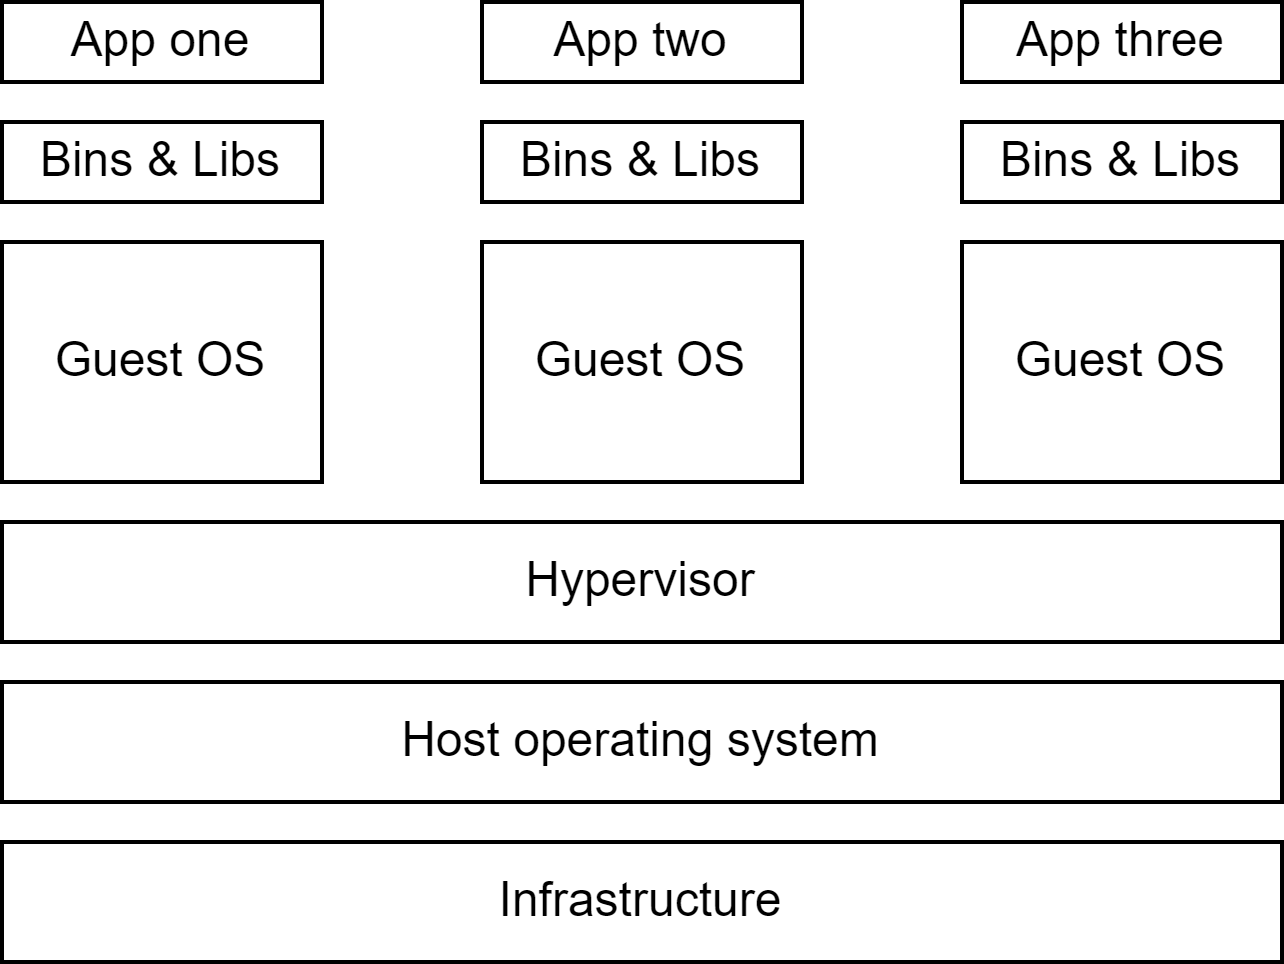
\includegraphics[width=0.5\linewidth]{images/vm.png}
    \caption{Virtual machine's structure}
\end{figure}
In this configuration, each operating system perceives the hardware as exclusively dedicated to itself. 
Virtualization results in significant power efficiency gains by consolidating the power consumption of individual machines, typically saving around 60\%.
Virtualization enables hot swaps, delivering two key advantages:
\begin{enumerate}
    \item \textit{Maintainability}.
    \item \textit{Availability}: overloaded machines can be supplemented by others.
\end{enumerate}

\subsection{Containers}
Containers encapsulate applications along with their dependencies into a uniform unit for streamlined software development and deployment.
\begin{figure}[H]
    \centering
    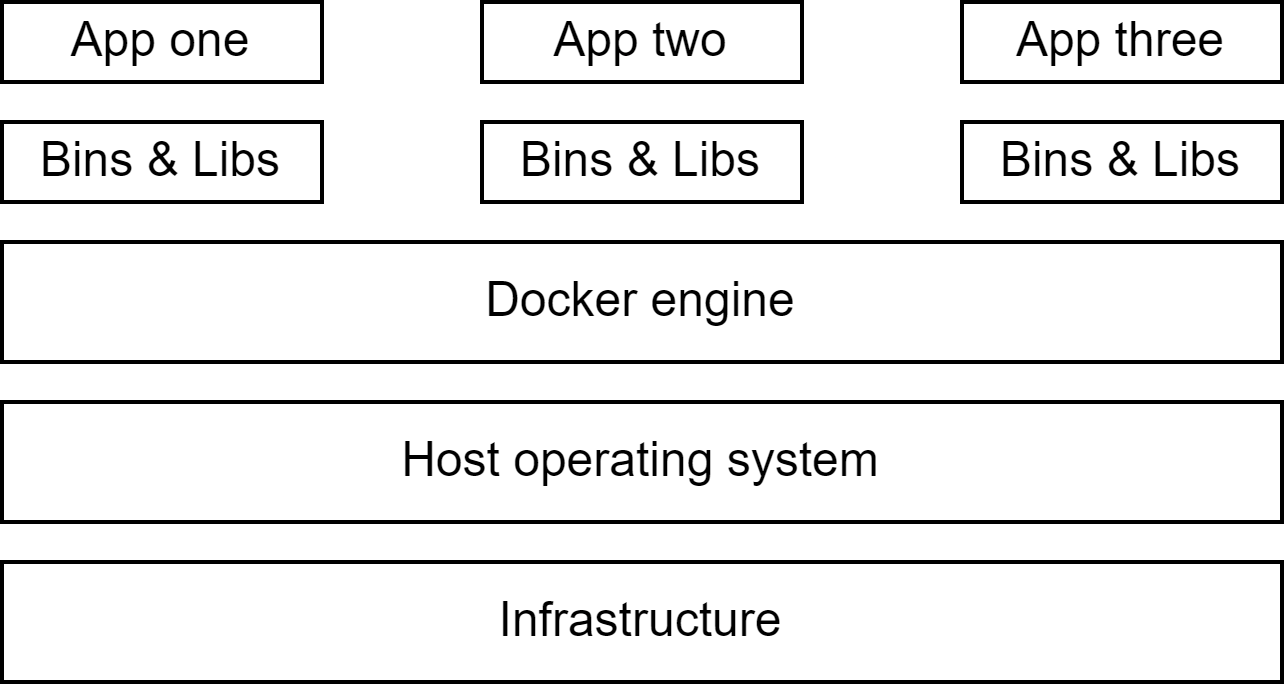
\includegraphics[width=0.5\linewidth]{images/container.png}
    \caption{Container's structure}
\end{figure}
Containers are employed to execute specific services and offer a lighter alternative to virtual machines.

\subsection{Summary}
Data centers offer several advantages, including reduced IT costs, enhanced performance, automatic software updates, seemingly limitless storage capacity, improved data reliability, universal document accessibility, and freedom from device constraints. 
However, it also presents challenges such as the need for a stable internet connection, poor compatibility with slow connections, limited hardware capabilities, privacy and security concerns, increased power consumption, and delays in decision-making.